\documentclass[12pt]{article}
\usepackage[spanish,es-noshorthands,es-nodecimaldot]{babel}
\usepackage{natbib}
\usepackage{url}
\usepackage[utf8]{inputenc}   % utf8x de la plantilla da problemas con listings y hyperref
\usepackage[T1]{fontenc}
\usepackage{lmodern}
\usepackage{amsmath}
\usepackage{graphicx}
\graphicspath{{images/}{../resultados/}}   % en el repo: ../resultados/; en Overleaf: subir las figuras a images/
\usepackage{parskip}
\usepackage{fancyhdr}
\usepackage{booktabs}
\usepackage{float}
\usepackage{xcolor}
\usepackage{listings}
\usepackage{caption}
\usepackage[hidelinks]{hyperref}


\usepackage{vmargin}
\setmarginsrb{3 cm}{2.5 cm}{2.5 cm}{2.5 cm} {1 cm}{1.5 cm}{1 cm}{1.5 cm}
%\setmarginsrb{leftmargin}{topmargin}{rightmargin}{bottommargin}{headheight}{headsep}{footheight}{footskip}


\title{Desarrollo e implementación de aplicaciones de cómputo paralelo basado en CUDA C}        % Title
\author{Michael Lata \\ Jordi Romero \\ Kevin Andrés Morocho Remache}    % Author
\date{\today}                            % Date

\makeatletter
\let\thetitle\@title
\let\theauthor\@author
\let\thedate\@date
\makeatother

\pagestyle{fancy}
\fancyhf{}
\lhead{Convolución de imágenes en CPU y CUDA C}
\cfoot{\thepage}

% Lo marcado con \pendiente{} se completa con la corrida 2.
\newcommand{\pendiente}[1]{\textcolor{red}{\textbf{[PENDIENTE: #1]}}}
% Archivos de resultados: en el repo están en ../resultados/; en Overleaf se suben a images/
% o a la raíz del proyecto. Si una tabla falta, se muestra un aviso en rojo en vez de un error.
\newcommand{\existeresultado}[3]{%
  \IfFileExists{../resultados/#1}{#2}{\IfFileExists{images/#1}{#2}{\IfFileExists{#1}{#2}{#3}}}}
\newcommand{\tabla}[1]{%
  \IfFileExists{../resultados/#1}{\input{../resultados/#1}}{%
  \IfFileExists{images/#1}{\input{images/#1}}{%
  \IfFileExists{#1}{\input{#1}}{\pendiente{falta #1}}}}}
\newcommand{\repo}{\url{https://github.com/Whiteherobot/convolucion-cuda}}

\lstset{basicstyle=\ttfamily\small, columns=fullflexible, frame=single, breaklines=true,
        keywordstyle=\bfseries, language=C++, literate={á}{{\'a}}1 {é}{{\'e}}1 {í}{{\'i}}1
        {ó}{{\'o}}1 {ú}{{\'u}}1 {ñ}{{\~n}}1}


\begin{document}

\renewcommand{\listtablename}{Lista de Tablas}
\renewcommand{\tablename}{Tabla}
\renewcommand{\listfigurename}{Lista de Figuras}
\renewcommand{\figurename}{Figura }

%%%%%%%%%%%%%%%%%%%%%%%%%%%%%%%%%%%%%%%%%%%%%%%%%%%%%%%%%%%%%%%%%%%%%%%%%%%%%%%%%%%%%%%%%
%%%%%%%%%%%%%  INICIO PORTADA  %%%%%%%%%%%%%%%%%%%%%%%%%%%%%%%%%%%%%%%%%%%%%%%%%%%%%%%%%%
%%%%%%%%%%%%%%%%%%%%%%%%%%%%%%%%%%%%%%%%%%%%%%%%%%%%%%%%%%%%%%%%%%%%%%%%%%%%%%%%%%%%%%%%%
\begin{titlepage}
    \centering
    \IfFileExists{images/logo.png}{\includegraphics[width=0.5\linewidth]{logo.png}}{}\\[1.0 cm]
    \textsc{\LARGE Universidad Politécnica Salesiana}\\[2.0 cm]
    \textsc{\Large CP}\\[0.5 cm]
    \textsc{\large Computación Paralela}\\[0.5 cm]
    \rule{\linewidth}{0.2 mm} \\[0.4 cm]
    { \huge \bfseries \thetitle}\\
    \rule{\linewidth}{0.2 mm} \\[1.5 cm]

 \begin{flushleft} \large
    \emph{Autores:}\\
    \theauthor
 \end{flushleft}

  \begin{flushleft} \large
    \emph{Profesores:}\\
    Ing. Gabriel Leon \\
  \end{flushleft}

  \begin{flushleft} \normalsize
    Repositorio: \repo\\
    Commit de entrega: \pendiente{hash}
  \end{flushleft}

  \vfill

  {\large \thedate}

\end{titlepage}

%%%%%%%%%%%%%%%%%%%%%%%%%%%%%%%%%%%%%%%%%%%%%%%%%%%%%%%%%%%%%%%%%%%%%%%%%%%%%%%%%%%%%%%%%
%%%%%%%%%%%%%    FIN  PORTADA  %%%%%%%%%%%%%%%%%%%%%%%%%%%%%%%%%%%%%%%%%%%%%%%%%%%%%%%%%%
%%%%%%%%%%%%%%%%%%%%%%%%%%%%%%%%%%%%%%%%%%%%%%%%%%%%%%%%%%%%%%%%%%%%%%%%%%%%%%%%%%%%%%%%%

%%%%%%%%%%%%%%%%%%%%%%%%%%%%%%%%%%%%%%%%%%%%%%%%%%%%%%%%%%%%%%%%%%%%%%%%%%%%%%%%%%%%%%%%%
%%%%%%%%%%%%%  INICIO INDICE  %%%%%%%%%%%%%%%%%%%%%%%%%%%%%%%%%%%%%%%%%%%%%%%%%%%%%%%%%%
%%%%%%%%%%%%%%%%%%%%%%%%%%%%%%%%%%%%%%%%%%%%%%%%%%%%%%%%%%%%%%%%%%%%%%%%%%%%%%%%%%%%%%%%%

\tableofcontents  %GENERA TABLA DE CONTENIDOS (Remover %)
\pagebreak        %PARA HACER UN SALTO DE PAGINA (Remover %)

\listoftables  %GENERA LISTA DE TABLAS (Remover %)
%\pagebreak        %PARA HACER UN SALTO DE PAGINA (Remover %)

\listoffigures  %GENERA LISTA DE FIGURAS (Remover %)

\pagebreak

%%%%%%%%%%%%%%%%%%%%%%%%%%%%%%%%%%%%%%%%%%%%%%%%%%%%%%%%%%%%%%%%%%%%%%%%%%%%%%%%%%%%%%%%%
%%%%%%%%%%%%%    FIN  INDICE  %%%%%%%%%%%%%%%%%%%%%%%%%%%%%%%%%%%%%%%%%%%%%%%%%%%%%%%%%%
%%%%%%%%%%%%%%%%%%%%%%%%%%%%%%%%%%%%%%%%%%%%%%%%%%%%%%%%%%%%%%%%%%%%%%%%%%%%%%%%%%%%%%%%%

%%%%%%%%%%%%%%%%%%%%%%%%%%%%%%%%%%%%%%%%%%%%%%%%%%%%%%%%%%%%%%%%%%%%%%%%%%%%%%%%%%%%%%%%%
%%%%%%%%%%%%%    INICIO   TEXTO   %%%%%%%%%%%%%%%%%%%%%%%%%%%%%%%%%%%%%%%%%%%%%%%%%%%%%%%
%%%%%%%%%%%%%%%%%%%%%%%%%%%%%%%%%%%%%%%%%%%%%%%%%%%%%%%%%%%%%%%%%%%%%%%%%%%%%%%%%%%%%%%%%
% ───────────────────────────── 1 ─────────────────────────────
\section{Introducción}

Aplicar tres filtros de convolución (media, realce de nitidez y laplaciano) a imágenes en
escala de grises de $2000\times2000$, $4000\times4000$ y $6000\times6000$ píxeles, con una
versión secuencial en C/C++ que sirve de referencia y una versión en CUDA C donde cada hilo
calcula un píxel de salida \cite{cudaguide,sanders2010}. Sobre ambas se valida la corrección numérica y se mide cómo
influyen en el tiempo el volumen de datos (resolución), el trabajo por píxel (tamaño de
máscara), la configuración de hilos por bloque y las transferencias CPU--GPU.

% ───────────────────────────── 2 ─────────────────────────────
\section{Solución}

El programa es un único ejecutable, \texttt{convolucion}, organizado en modelo, vista y
controlador:

\begin{itemize}
  \item \textbf{Modelo} (\texttt{src/modelo}): lectura y escritura PGM (\texttt{imagen.cpp}),
        máscaras (\texttt{mascara.cpp}), convolución secuencial (\texttt{convolucion\_cpu.cpp})
        y convolución CUDA (\texttt{convolucion\_gpu.cu}).
  \item \textbf{Vista} (\texttt{src/vista}): impresión en consola y escritura del CSV.
  \item \textbf{Controlador} (\texttt{src/controlador}): \texttt{main.cu} con tres modos
        (\texttt{filtrar}, \texttt{probar}, \texttt{medir}), las pruebas de corrección
        (\texttt{pruebas.cu}) y los experimentos (\texttt{experimentos.cu}).
\end{itemize}

Condiciones comunes a CPU y GPU: imágenes en grises de 8 bits leídas a \texttt{float},
mismas máscaras en \texttt{float}, extensión con ceros fuera de la imagen y arreglos
separados de entrada y salida. Se calcula como correlación (sin invertir la máscara); como
las tres máscaras son simétricas respecto de su centro, el resultado coincide con el de la
convolución.

\paragraph{Conversión al rango de visualización.} Todo el cálculo y la validación se hacen
en \texttt{float}. Solo al guardar el PGM (\texttt{guardar\_pgm}) cada valor se recorta a
$[0,255]$ y se redondea (\texttt{a\_rango\_visual}). Esta conversión pierde información en los
filtros que producen valores fuera del rango (sección~\ref{sec:imagenes}).

% ───────────────────────────── 3 ─────────────────────────────
\section{Filtros y máscaras}

\begin{table}[H]
\centering
\caption{Máscaras utilizadas.}
\begin{tabular}{lcl}
\toprule
Filtro & Máscara & Efecto \\
\midrule
Media $k\times k$ ($k=3,9,21$) & todos los coeficientes $= \dfrac{1}{k^2}$ &
  Suaviza: promedia la vecindad \\[2ex]
Nitidez $3\times3$ & $\begin{bmatrix}0&-1&0\\-1&5&-1\\0&-1&0\end{bmatrix}$ &
  Realza bordes y detalles \\[4ex]
Laplaciano $3\times3$ & $\begin{bmatrix}0&1&0\\1&-4&1\\0&1&0\end{bmatrix}$ &
  Resalta cambios de intensidad \\
\bottomrule
\end{tabular}
\end{table}

Las máscaras siguen las definiciones habituales de filtrado espacial \cite{gonzalez2018}. La media suma 1, por lo que conserva el brillo medio y su salida queda siempre en $[0,255]$.
La nitidez equivale a la imagen original menos su laplaciano (suma 1): conserva las zonas
uniformes y amplifica las diferencias con los vecinos. El laplaciano suma 0: en zonas
uniformes da 0 y en los bordes da valores positivos o negativos según el lado del cambio.

% ───────────────────────────── 4 ─────────────────────────────
\section{Distribución del trabajo en la GPU}

Se usan bloques e hilos solo en la dimensión X. La imagen de $\textit{ancho}\times\textit{alto}$
se trata como un arreglo lineal de $n=\textit{ancho}\cdot\textit{alto}$ píxeles almacenado por
filas, y cada hilo calcula un píxel de salida leyendo la entrada y la máscara desde memoria
global:

\begin{lstlisting}
int tid = blockIdx.x * blockDim.x + threadIdx.x;  // índice global del hilo
if (tid < ancho * alto) {                          // el último bloque puede sobrar
    fila    = tid / ancho;
    columna = tid % ancho;
    for (i = 0; i < k; i++)
        for (j = 0; j < k; j++) {
            int y = fila + i - radio, x = columna + j - radio;
            if (y >= 0 && y < alto && x >= 0 && x < ancho)   // ceros fuera
                suma += entrada[y * ancho + x] * mascara[i * k + j];
        }
    salida[tid] = suma;
}
\end{lstlisting}

El número de bloques se ajusta para cubrir la imagen:
$\textit{bloques} = \lceil n / \textit{hilos} \rceil = (n + \textit{hilos} - 1) / \textit{hilos}$.
Los hilos con $\textit{tid} \ge n$ no hacen nada. Por ejemplo, la imagen de prueba de
$1001\times777$ tiene $777\,777$ píxeles; con 256 hilos por bloque se lanzan 3039 bloques
($777\,984$ hilos) y 207 hilos del último bloque quedan inactivos. Las imágenes de los
experimentos sí son múltiplos (por ejemplo, $4000^2/256 = 62\,500$ bloques), por eso la prueba
con $1001\times777$ es la que ejercita el control de límites.

% ───────────────────────────── 5 ─────────────────────────────
\section{Equipo y herramientas}

Las mediciones se ejecutaron en el equipo de Michael Lata. Datos tomados de
\texttt{resultados/equipo.txt} (generado por \texttt{scripts/info\_equipo.sh}):

\begin{table}[H]
\centering
\caption{Equipo de medición.}
\begin{tabular}{ll}
\toprule
CPU & Intel Core i7-13650HX, 14 núcleos, 20 hilos \\
RAM & 15 GiB \\
GPU & NVIDIA GeForce RTX 4060 Laptop GPU, 8188 MiB \\
Driver NVIDIA & 615.78.08 \\
CUDA & 13.4 (\texttt{nvcc} build \texttt{cuda\_13.4.r13.4}) \\
Compilador host & GCC 16.2.1 \\
CMake & 4.4.5 \\
Python & 3.14.8 \\
Sistema & Linux 7.3.0-4-cachyos x86\_64 \\
Compilación & CMake en modo Release, arquitectura CUDA \texttt{native} \\
\bottomrule
\end{tabular}
\end{table}

% ───────────────────────────── 6 ─────────────────────────────
\section{Preparación de datos}

Las tres resoluciones se obtienen de la misma fotografía, \texttt{datos/original.jpg}
($6200\times8272$), con \texttt{scripts/preparar\_imagenes.py}: conversión a grises, recorte
cuadrado centrado de $6200\times6200$ (desde la fila 1036) y reducción con LANCZOS a 6000, 4000
y 2000 píxeles de lado. No hay ampliación. Todas las implementaciones leen exactamente los
mismos archivos \texttt{datos/imagen\_\{2000,4000,6000\}.pgm}.

% ───────────────────────────── 7 ─────────────────────────────
\section{Metodología de medición}

\begin{table}[H]
\centering
\caption{Experimentos. Se modifica un factor a la vez.}
\begin{tabular}{clll}
\toprule
Exp. & Varía & Fijo & Configuraciones \\
\midrule
1 & Filtro & $4000\times4000$, $3\times3$, 256 hilos & media, nitidez, laplaciano \\
2 & Resolución & media $9\times9$, 256 hilos & 2000, 4000, 6000 \\
3 & Máscara & media, $4000\times4000$, 256 hilos & $k=3, 9, 21$ \\
4 & Hilos por bloque & media $9\times9$, $4000\times4000$ & 128, 256, 512 \\
\bottomrule
\end{tabular}
\end{table}

\begin{itemize}
  \item \textbf{Orden por configuración}: primero la CPU (una ejecución de calentamiento
        y 5 medidas seguidas), luego un calentamiento de la GPU de al menos 2\,s de trabajo
        continuo y después las 5 repeticiones GPU seguidas. Los tiempos se guardan en
        memoria y el CSV se escribe al final, para no dejar a la GPU sin trabajo entre
        repeticiones.
  \item \textbf{Por qué este orden}: en las corridas 1 y 2, CPU y GPU se alternaban en
        cada repetición con un solo calentamiento GPU. Mientras la CPU calculaba, la GPU de
        la laptop quedaba sin trabajo y bajaba de reloj y de enlace PCIe, así que la misma
        configuración dio tiempos de kernel hasta 8 veces distintos
        (sección~\ref{sec:limitaciones}). La CPU es estable (variación menor al 3\,\%), por lo
        que medirla en bloque no altera sus resultados.
  \item \textbf{Repeticiones}: 5 medidas por implementación y configuración. Cada
        experimento mide sus propias configuraciones aunque coincidan con las de otro (media
        $9\times9$, 4000, 256 hilos aparece en los experimentos 2, 3 y 4).
  \item \textbf{Validación}: la salida de la última repetición GPU medida se compara con la
        de la CPU (error absoluto máximo y medio, tolerancia $10^{-3}$).
  \item \textbf{Estadísticos}: mediana como valor central; desviación estándar, mínimo y
        máximo como variabilidad.
  \item \textbf{CPU}: solo la llamada a \texttt{convolucion\_cpu}, con
        \texttt{std::chrono::steady\_clock}.
  \item \textbf{GPU}: eventos CUDA en el flujo por defecto. CPU$\to$GPU (imagen y máscara),
        kernel y GPU$\to$CPU se miden entre eventos consecutivos y el total va del primer
        al último evento. Se espera con \texttt{cudaEventSynchronize} antes de leer los
        tiempos.
  \item \textbf{Fuera de la medición}: lectura y escritura de archivos, preparación de
        imágenes y máscaras, escritura del CSV y la reserva y liberación de memoria
        (\texttt{cudaMalloc} y \texttt{cudaFree} quedan fuera de los eventos). La memoria del
        host es paginable (\texttt{malloc}).
  \item \textbf{Aceleración}: de cómputo $= T_{CPU}/T_{kernel}$; con transferencias
        $= T_{CPU}/T_{total\,GPU}$, ambas con medianas.
  \item \textbf{Registro}: \texttt{resultados/mediciones.csv}, una fila por implementación y
        repetición con experimento, filtro, resolución, máscara, hilos por bloque, bloques,
        repetición, tiempos y unidad (ms). \texttt{scripts/graficas.py} genera a partir de él
        el resumen, las tablas y las gráficas.
\end{itemize}

% ───────────────────────────── 8 ─────────────────────────────
\section{Validación}

\subsection{Prueba manual}
Se usa la matriz $5\times5$ y la máscara $3\times3$ de la figura 1 del enunciado. Los
valores esperados se calcularon a mano; por ejemplo, para el píxel (1,1):
$35(-2)+40(-1)+41(0)+40(-1)+40(1)+42(1)+42(0)+46(1)+50(2)=78$. En la esquina (0,0) solo
cuatro vecinos están dentro de la imagen: $35(1)+40(1)+40(1)+40(2)=195$. CPU y GPU obtienen
exactamente 78, 87 y 195 (\texttt{resultados/prueba.txt}).

\subsection{Comparación numérica CPU--GPU}
Se compara la salida en \texttt{float}, antes de convertirla a $[0,255]$, píxel a píxel:
$e_{max}=\max_i |c_i-g_i|$ y $\bar e = \frac1n\sum_i |c_i-g_i|$.

\begin{table}[H]
\centering
\caption{Error absoluto CPU vs GPU (de \texttt{prueba.txt} y \texttt{medir\_consola.txt}).}
\begin{tabular}{llrr}
\toprule
Imagen & Máscara & $e_{max}$ & $\bar e$ \\
\midrule
$1001\times777$ aleatoria, 256 hilos & media $3\times3$ & $4.58\times10^{-5}$ & $2.96\times10^{-6}$ \\
 & media $9\times9$ & $4.58\times10^{-5}$ & $3.78\times10^{-6}$ \\
 & nitidez & 0 & 0 \\
 & laplaciano & 0 & 0 \\
\midrule
$4000\times4000$ & media $3\times3$ & $4.58\times10^{-5}$ & $3.04\times10^{-6}$ \\
 & media $9\times9$ (128, 256, 512 hilos) & $1.07\times10^{-4}$ & $5.21\times10^{-6}$ \\
 & media $21\times21$ & $1.07\times10^{-4}$ & $4.19\times10^{-6}$ \\
 & nitidez, laplaciano & 0 & 0 \\
$2000\times2000$ & media $9\times9$ & $9.16\times10^{-5}$ & $5.21\times10^{-6}$ \\
$6000\times6000$ & media $9\times9$ & $1.22\times10^{-4}$ & $5.19\times10^{-6}$ \\
\bottomrule
\end{tabular}
\end{table}

La imagen de $1001\times777$ no es múltiplo de 256 y valida el control de límites del último
bloque. Con imágenes reales las 12 configuraciones de los experimentos se comparan antes de
medir y todas quedan dentro de la tolerancia.

\paragraph{Tolerancia: $10^{-3}$ en valor absoluto.} Nitidez y laplaciano tienen coeficientes
enteros y entradas enteras, sus productos y sumas son exactos en \texttt{float} y el error es
exactamente 0. La media usa $1/k^2$, que no es representable exactamente; la diferencia
aparece por el redondeo de las operaciones en coma flotante, probablemente porque el
compilador de CUDA contrae multiplicación y suma en una sola operación (FMA) mientras que la
CPU las redondea por separado. Un error de este origen es del orden del épsilon de
\texttt{float} ($\approx1.2\times10^{-7}$) por el valor acumulado ($\le255$), es decir, alrededor
de $10^{-5}$ a $10^{-4}$, como se observa. La tolerancia $10^{-3}$ deja margen sobre ese orden y
es 500 veces menor que 0.5, la mínima diferencia que podría cambiar un píxel al redondear a
entero; por debajo de ella, CPU y GPU producen la misma imagen visible salvo empates exactos
en el redondeo. El mayor error observado ($1.22\times10^{-4}$) está 8 veces por debajo de la
tolerancia.

\subsection{Verificación independiente de rangos}
\texttt{scripts/figuras\_filtros.py} repite la convolución con una implementación propia en
\texttt{numpy} (extensión con ceros) para calcular los rangos de la tabla~\ref{tab:rangos}.
Coincide con los valores que reporta la implementación en C sobre las mismas imágenes.

% ───────────────────────────── 9 ─────────────────────────────
\section{Imágenes representativas}\label{sec:imagenes}

\begin{figure}[H]
\centering
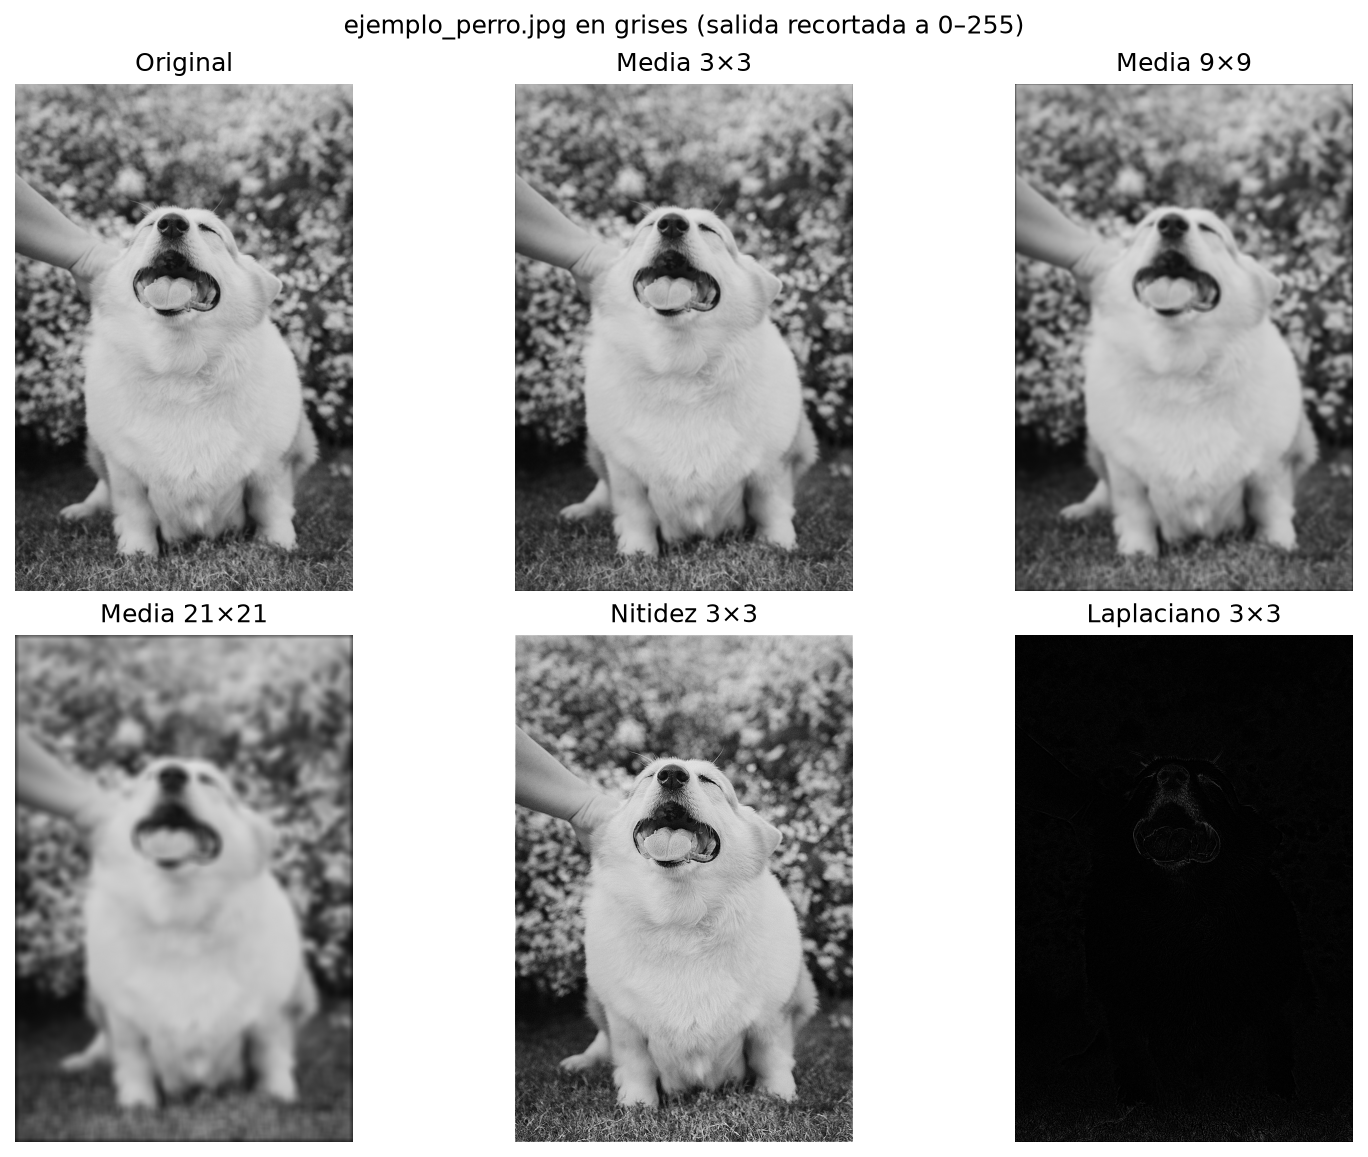
\includegraphics[width=0.92\textwidth]{figura_filtros_perro.png}
\caption{Filtros sobre \texttt{ejemplo\_perro.jpg} en grises ($800\times1200$).}
\end{figure}

\begin{figure}[H]
\centering
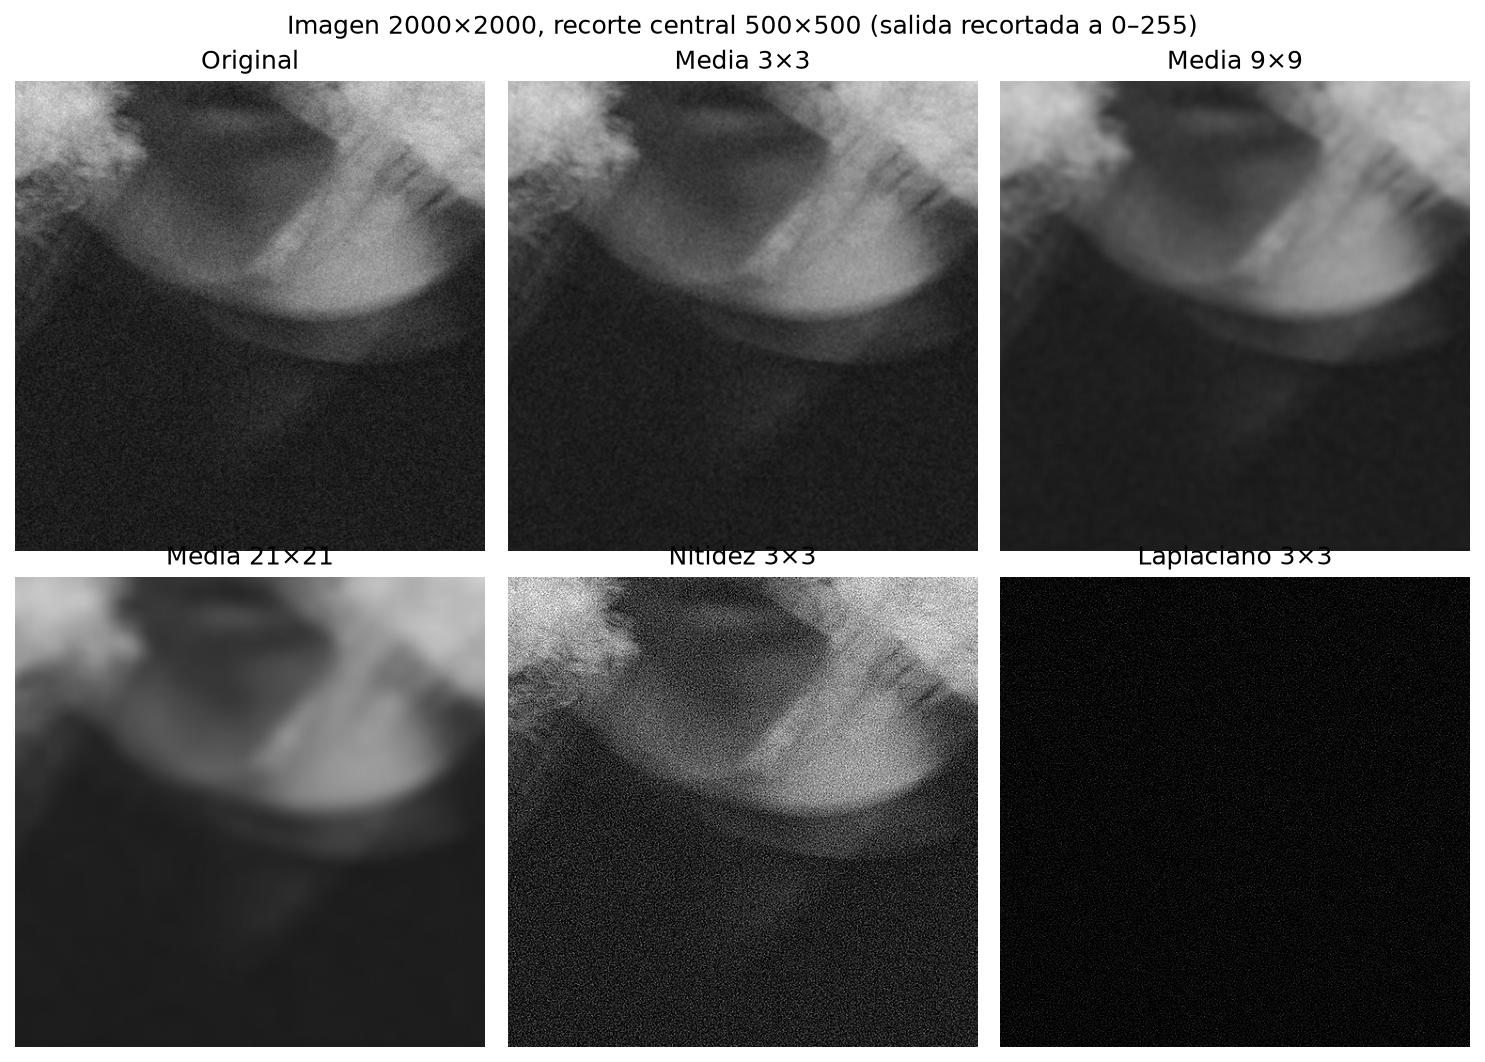
\includegraphics[width=0.92\textwidth]{figura_filtros_imagen.png}
\caption{Filtros sobre un recorte central de $500\times500$ de la imagen de 2000.}
\end{figure}

\begin{table}[H]
\centering
\caption{Rango de la salida en \texttt{float} antes de convertir a $[0,255]$
(\texttt{resultados/rangos\_filtros.csv}).}\label{tab:rangos}
\begin{tabular}{llrrrr}
\toprule
Imagen & Filtro & Mín. & Máx. & \% $<0$ & \% $>255$ \\
\midrule
imagen 2000 & media 3/9/21 & 9.4 / 13.1 / 13.1 & 244.0 / 233.7 / 229.9 & 0 & 0 \\
 & nitidez & $-91.0$ & 724.0 & 3.9 & 2.4 \\
 & laplaciano & $-488.0$ & 114.0 & 49.0 & 0 \\
ejemplo\_perro & nitidez & $-209.0$ & 583.0 & 0.4 & 0.2 \\
 & laplaciano & $-389.0$ & 229.0 & 48.3 & 0 \\
\bottomrule
\end{tabular}
\end{table}

La media nunca sale de $[0,255]$ y la conversión no la altera. La nitidez supera el rango en
ambos sentidos en pocos píxeles (bordes muy marcados) y el recorte los satura. En el
laplaciano casi la mitad de los píxeles son negativos: el recorte a 0 los convierte en negro y
solo quedan visibles los bordes del lado positivo, por eso la imagen se ve casi negra. Es un
efecto de la conversión elegida, no del cálculo, que se validó antes de convertir.

\begin{figure}[H]
\centering
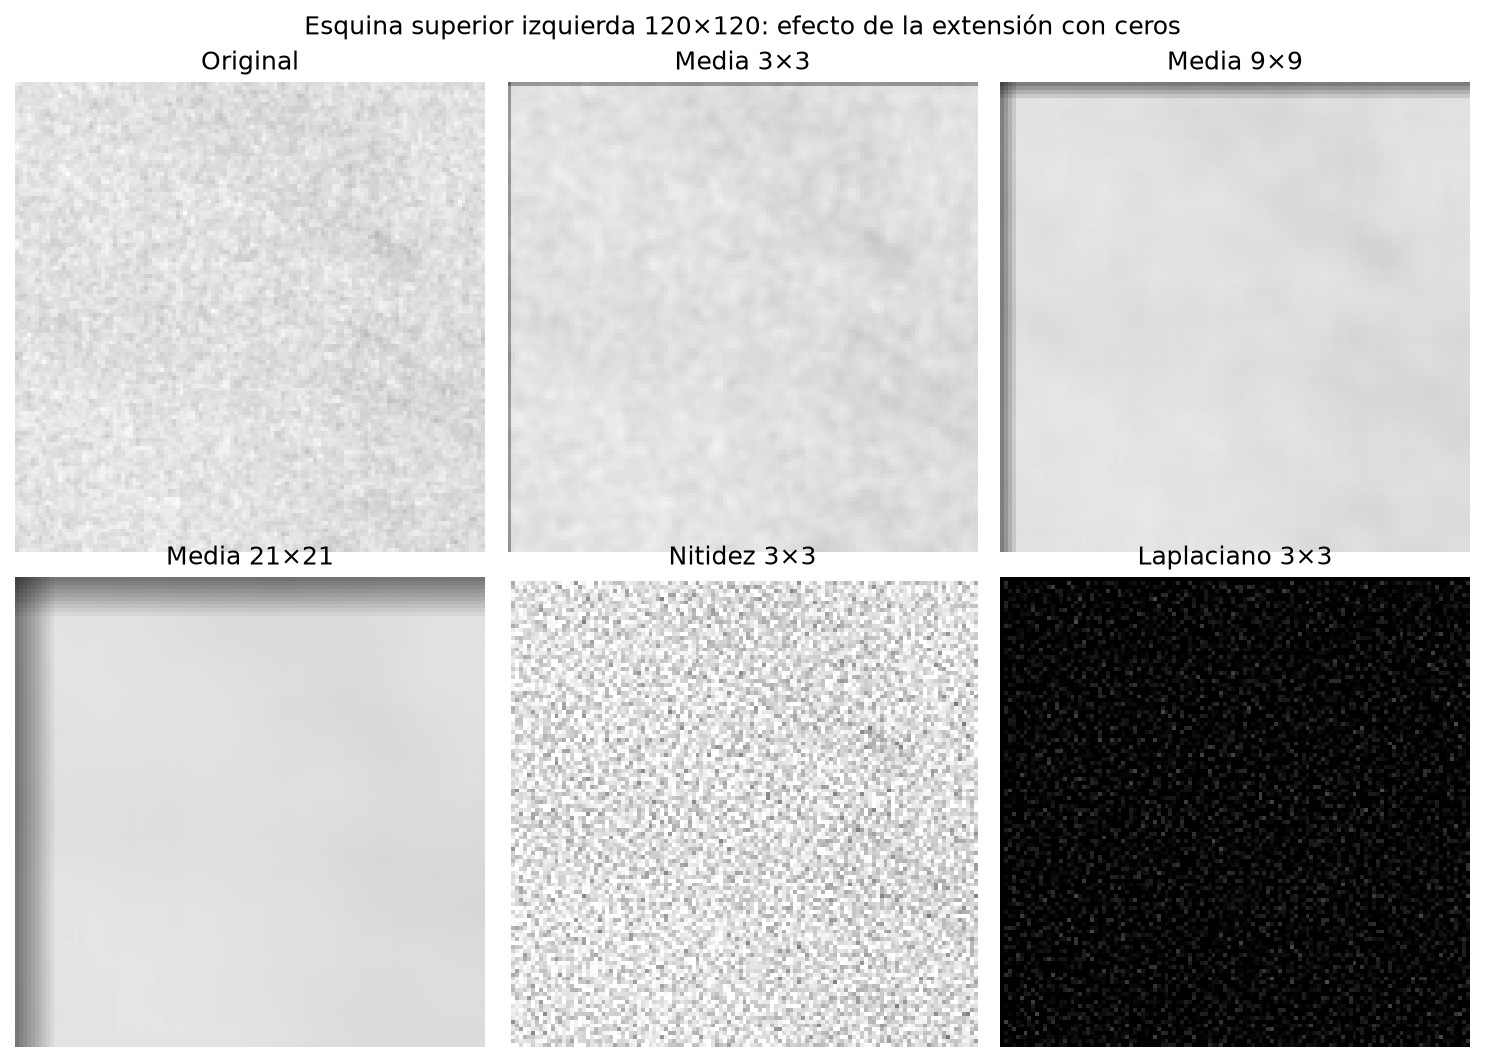
\includegraphics[width=0.8\textwidth]{figura_bordes.png}
\caption{Esquina de la imagen de 2000: la extensión con ceros oscurece una franja de
$\lfloor k/2\rfloor$ píxeles (1, 4 y 10 para $k=3,9,21$), porque los vecinos fuera de la imagen
aportan 0 al promedio.}
\end{figure}

% ───────────────────────────── 10 ─────────────────────────────
\section{Resultados}

\subsection{Corrida 1: tiempos con dos niveles de rendimiento}

En la primera corrida (\texttt{resultados/mediciones\_corrida1.csv}) la CPU fue estable
(desviación estándar entre 1 y 3\,\% de la mediana), pero los tiempos de GPU de una misma
configuración tomaron valores discretos muy distintos. La figura~\ref{fig:rep1} muestra las 60
repeticiones GPU en orden de ejecución:

\begin{itemize}
  \item La copia CPU$\to$GPU alterna entre dos niveles, $\approx3.2$ y $\approx1.6$ GB/s,
        exactamente la mitad, sin valores intermedios, y en todos los experimentos.
  \item El kernel también cambia por escalones: media $9\times9$ en 4000 tarda 11.7, 13.0,
        19.7, 26.1 o 33.5\,ms con el mismo cálculo, y valores como 33.51 y 26.07\,ms se repiten
        exactamente varias veces.
  \item Al mismo tiempo la CPU no cambia, por lo que no es otro proceso compitiendo por la
        CPU: el cambio está en la GPU o en el bus PCIe.
\end{itemize}

\begin{figure}[H]
\centering
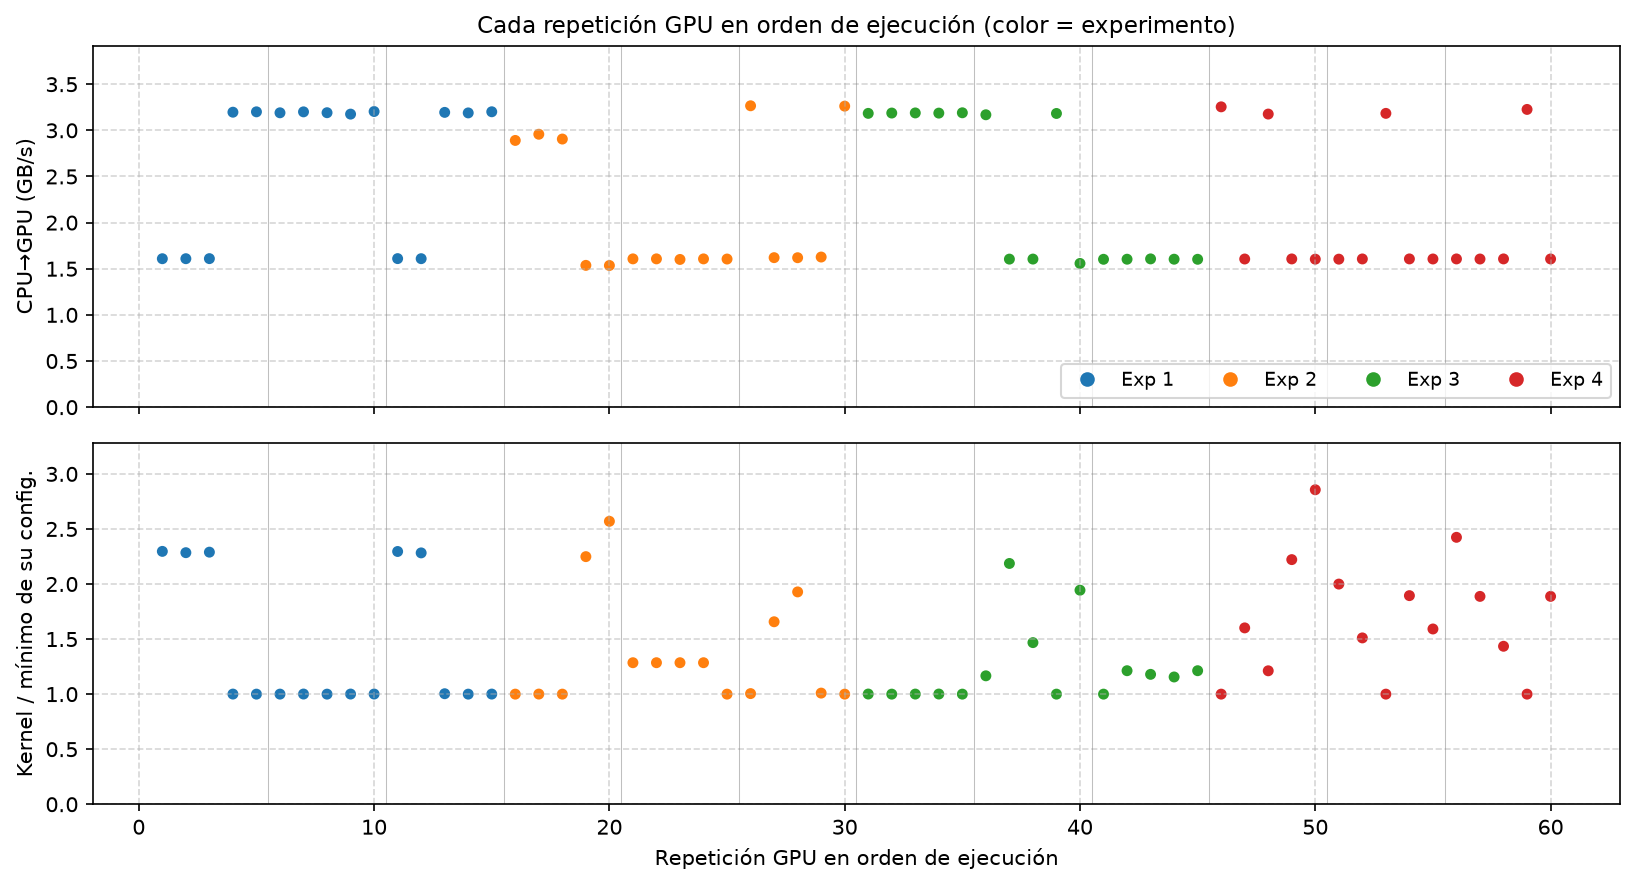
\includegraphics[width=\textwidth]{grafica_repeticiones_corrida1.png}
\caption{Corrida 1: cada repetición GPU en orden de ejecución.}\label{fig:rep1}
\end{figure}

Valores exactos que se repiten y una relación exacta de 2 en el ancho de banda son
compatibles con cambios de estado de energía de la GPU portátil (frecuencia de reloj y
velocidad del enlace PCIe), que no se registraron en esa corrida. Por eso se repitió la medición
registrando el estado de la GPU con \texttt{nvidia-smi} (\texttt{resultados/gpu\_estado.csv}).
\pendiente{confirmar o descartar con gpu\_estado.csv de la corrida 2}

Consecuencias en la corrida 1: en el experimento 1 el kernel de la media $3\times3$ aparece 2.3 veces más
lento que el de nitidez y laplaciano porque 3 de sus 5 repeticiones cayeron en el nivel lento (en el
experimento 3 la misma configuración da 5.45\,ms en las 5); y en el experimento 4 la diferencia
entre configuraciones de hilos es menor que la diferencia entre niveles, por lo que no permite
elegir una. La tabla completa de la corrida 1 está en el anexo~\ref{sec:anexo}.

\subsection{Corrida 2}

\existeresultado{tabla_resumen.tex}{
\begin{table}[H]
\centering
\small
\caption{Corrida 2: medianas de 5 repeticiones y variabilidad.}
\resizebox{\textwidth}{!}{\tabla{tabla_resumen.tex}}
\end{table}
\begin{figure}[H]\centering
\includegraphics[width=\textwidth]{grafica_repeticiones.png}
\caption{Corrida 2: cada repetición GPU en orden de ejecución.}\end{figure}
\begin{figure}[H]\centering
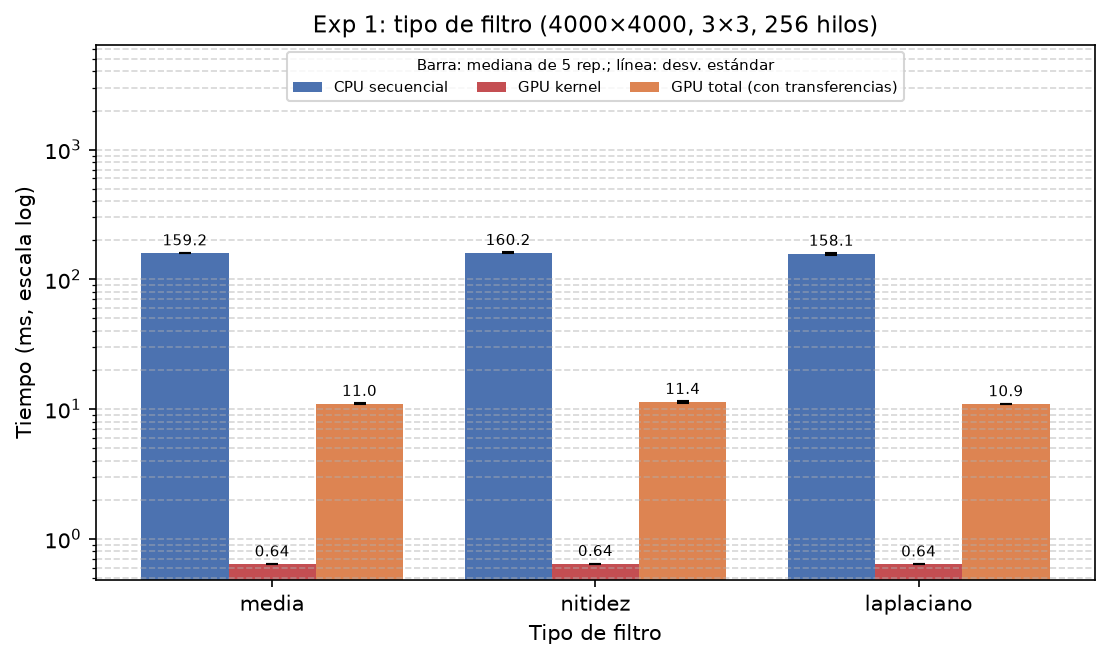
\includegraphics[width=0.49\textwidth]{grafica_exp1_filtros.png}
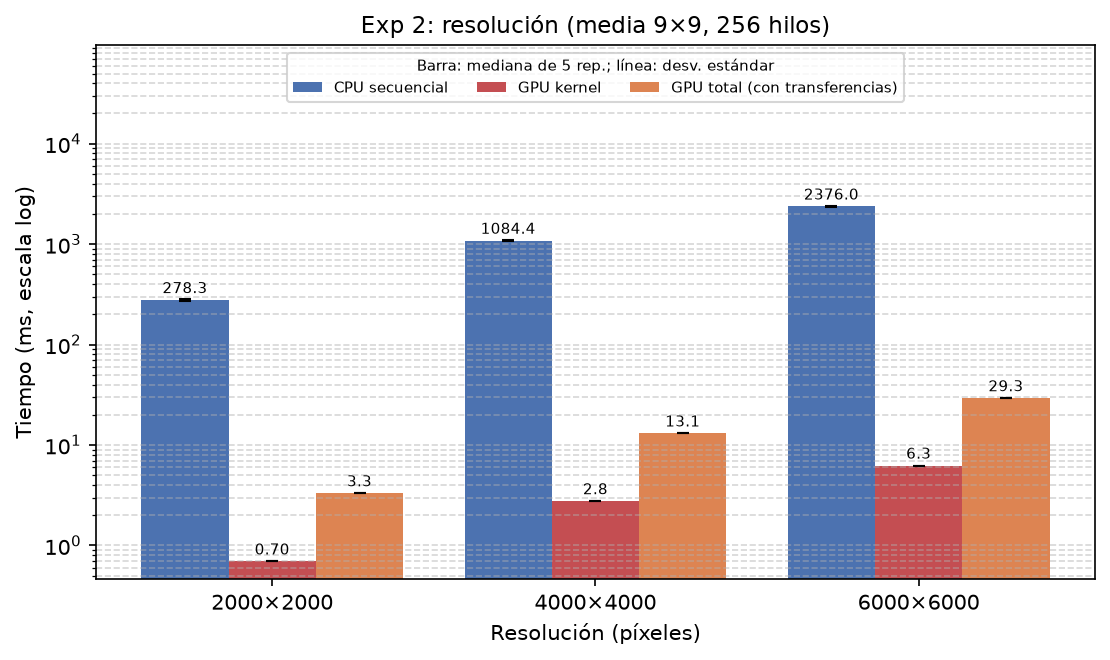
\includegraphics[width=0.49\textwidth]{grafica_exp2_resolucion.png}
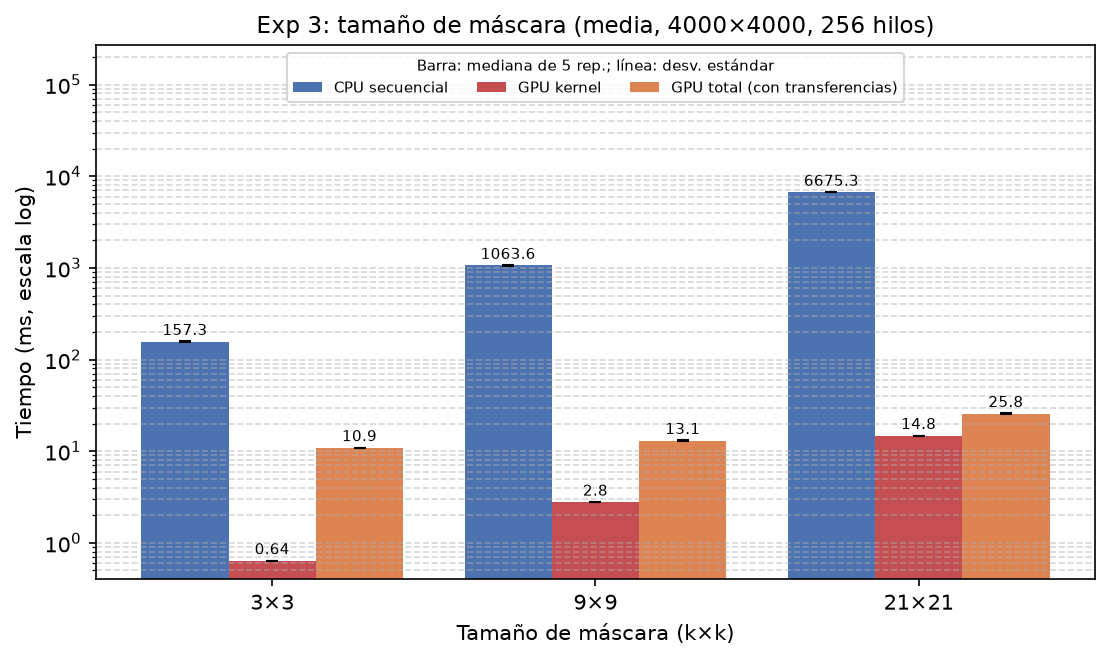
\includegraphics[width=0.49\textwidth]{grafica_exp3_mascara.png}
\caption{Corrida 2: CPU, kernel y total GPU por experimento (escala logarítmica).}\end{figure}
\begin{figure}[H]\centering
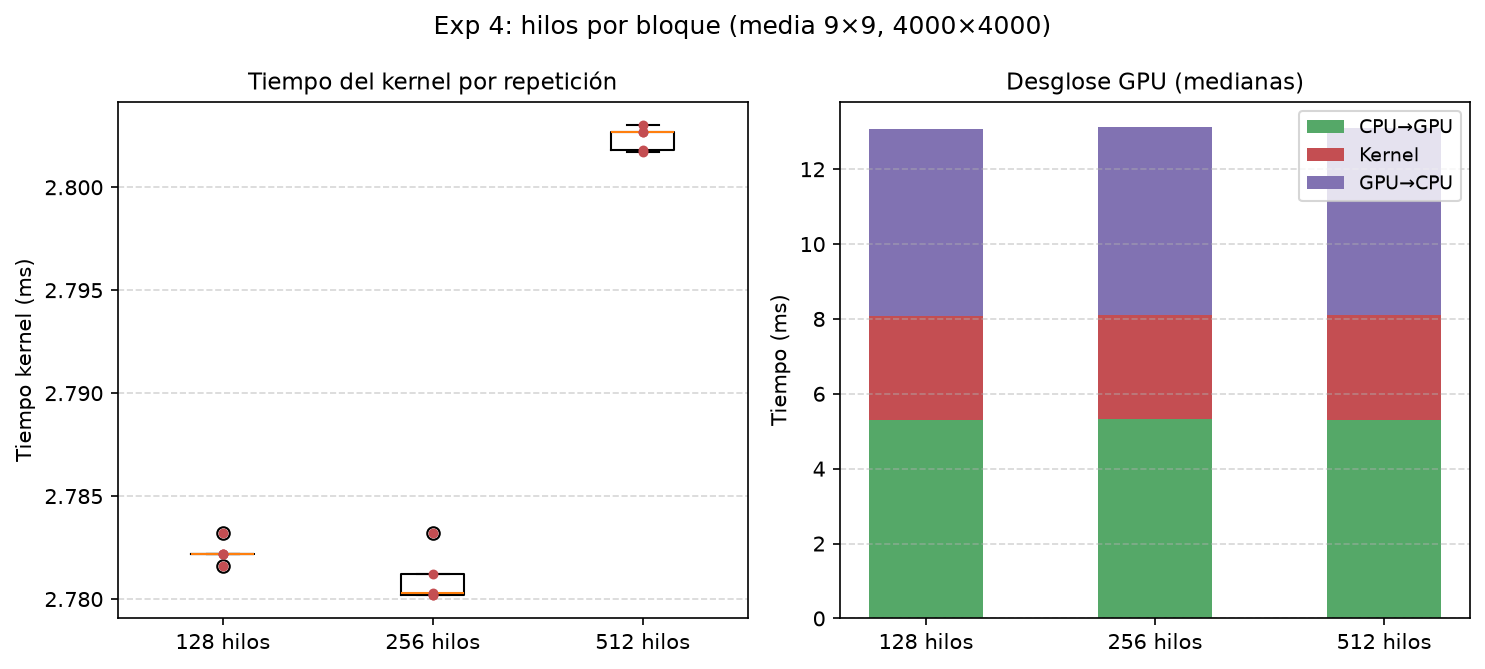
\includegraphics[width=\textwidth]{grafica_exp4_hilos.png}
\caption{Corrida 2: hilos por bloque.}\end{figure}
\begin{figure}[H]\centering
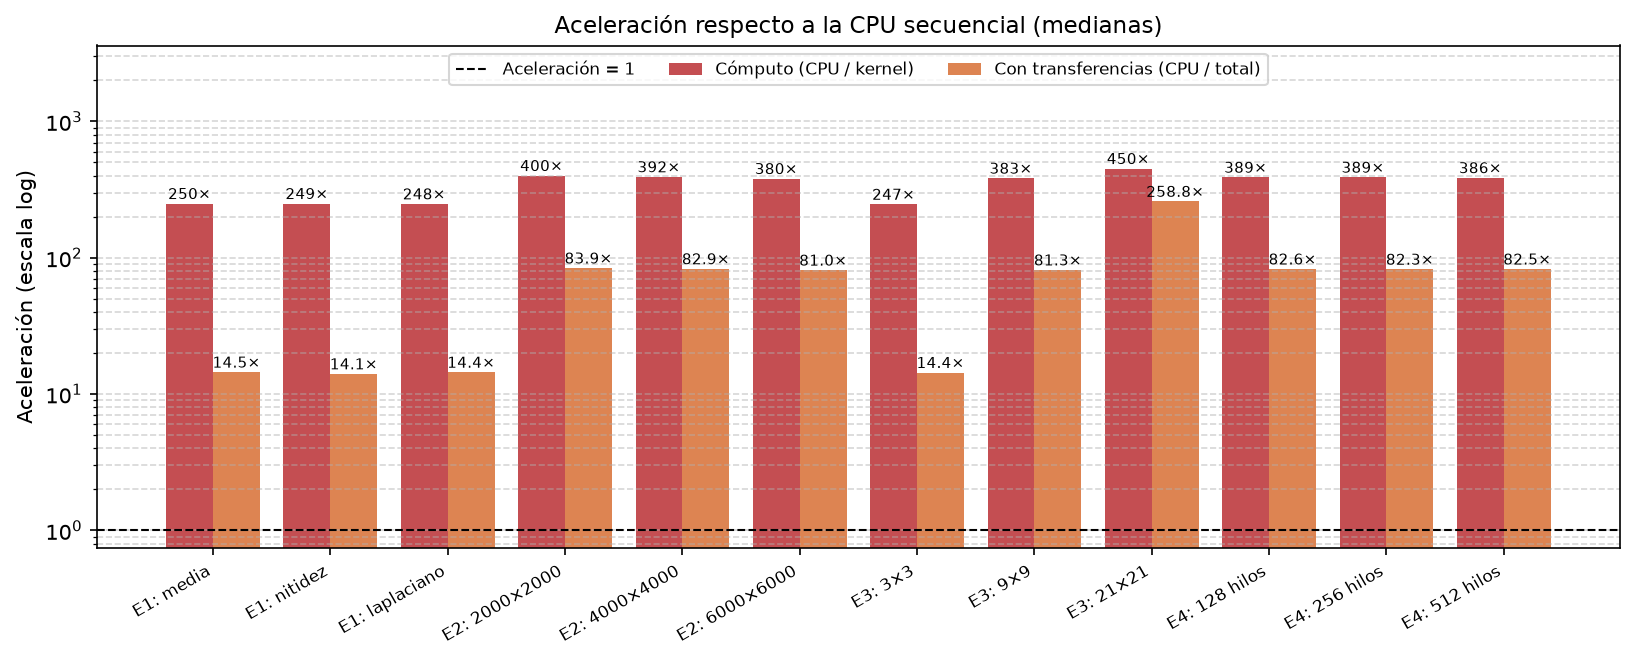
\includegraphics[width=\textwidth]{grafica_speedup.png}
\caption{Corrida 2: aceleración de cómputo y con transferencias.}\end{figure}
\begin{figure}[H]\centering
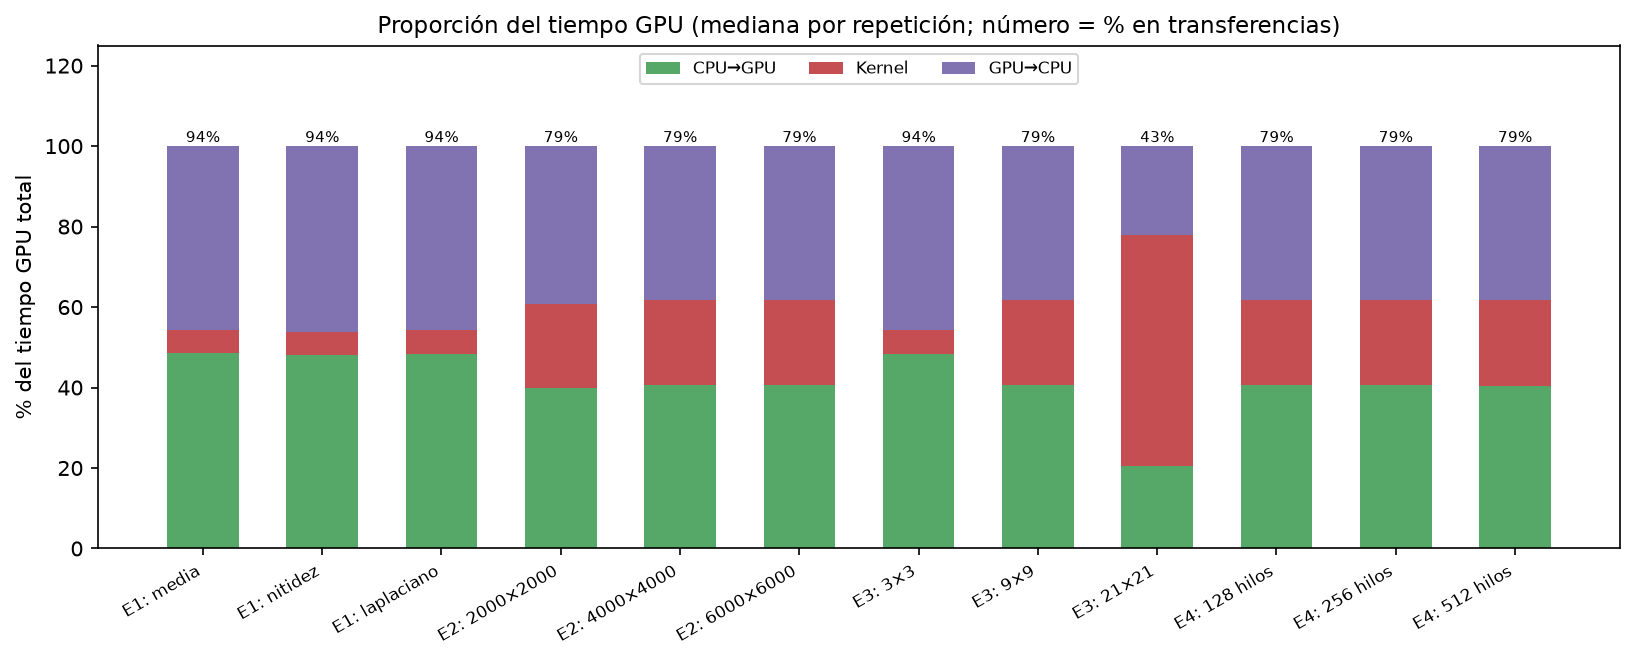
\includegraphics[width=\textwidth]{grafica_gpu_desglose.png}
\caption{Corrida 2: proporción del tiempo GPU.}\end{figure}
}{\pendiente{tabla y gráficas de la corrida 2: ejecutar \texttt{python3 scripts/graficas.py}}}

% ───────────────────────────── 11 ─────────────────────────────
\section{Análisis}

\subsection{¿Cómo cambia el tiempo con la resolución y el tamaño de máscara?}

\textbf{CPU.} El trabajo es $n\cdot k^2$ multiplicaciones y sumas, y el tiempo de CPU lo
sigue de cerca. Resolución (media $9\times9$): 263.9, 1073.6 y 2420.1\,ms para 2000, 4000 y
6000; con 4 y 9 veces más píxeles, el tiempo crece 4.07 y 9.17 veces. Máscara (4000): 153.0,
1092.6 y 6781.7\,ms para $k=3, 9, 21$; con $k^2$ 9 y 49 veces mayor, el tiempo crece 7.1 y
44.3 veces. El costo por operación queda entre 0.82 y 1.10\,ns en todas las configuraciones
(corrida 1, en la que la CPU fue estable). El tipo de filtro no cambia el tiempo con la misma
máscara: 153.6, 158.8 y 155.9\,ms para media, nitidez y laplaciano $3\times3$, diferencias del
orden de su desviación estándar (3.2--4.7\,ms).

\textbf{GPU.} \pendiente{con la corrida 2: crecimiento del kernel y de las transferencias con
$n$ y con $k^2$}. Las transferencias dependen solo de $n$ (no de $k$), mientras que el kernel
depende de $n\cdot k^2$.

\subsection{¿Qué proporción del tiempo GPU corresponde a transferencias?}

En la corrida 1, calculando el porcentaje en cada repetición, las transferencias son entre
86 y 88\,\% del tiempo GPU con máscaras $3\times3$, entre 69 y 81\,\% con $9\times9$ en todas
las resoluciones, y entre 21 y 35\,\% con $21\times21$. Con $3\times3$ la proporción casi no
cambia entre los dos niveles de rendimiento (86.2\,\% en el lento y 87.8\,\% en el rápido)
porque copias y kernel se ralentizan juntos. Con poco trabajo por
píxel la GPU pasa la mayor parte del tiempo copiando datos; solo con la máscara $21\times21$
el cómputo domina. \pendiente{confirmar con la corrida 2}

\subsection{¿Qué configuración de hilos por bloque es mejor y qué variabilidad presenta?}

En la corrida 1 los kernels de 128, 256 y 512 hilos tienen medianas de 18.8, 20.7 y
26.2\,ms, pero cada configuración va de $\approx12$ a $\approx34$\,ms entre repeticiones por los
cambios de nivel: la variabilidad supera a la diferencia entre configuraciones y no se puede
concluir cuál es mejor. \pendiente{corrida 2: mediana, desviación y rango de cada configuración}

\subsection{¿Qué confirma o contradice las expectativas?}

\begin{itemize}
  \item \textbf{Esperado y confirmado}: el tiempo de CPU es proporcional a $n\cdot k^2$; el
        tipo de filtro no influye con la misma máscara; la GPU calcula el mismo resultado que
        la CPU dentro de la tolerancia.
  \item \textbf{Esperado y confirmado}: las transferencias limitan la aceleración real con
        máscaras pequeñas; la aceleración con transferencias es muy inferior a la de
        cómputo (corrida 1: $\approx3.5\times$ frente a $\approx29\times$ con $3\times3$).
  \item \textbf{No esperado}: tiempos de GPU con dos niveles en la corrida 1. La evidencia
        (figura~\ref{fig:rep1}) son valores discretos repetidos y un ancho de banda que cae
        exactamente a la mitad, con la CPU estable.
  \item \textbf{No esperado}: el ancho de banda CPU$\to$GPU (3.2\,GB/s en el mejor caso) es
        bajo para PCIe; es coherente con copiar desde memoria paginable, que obliga al driver
        a pasar por un búfer intermedio \cite{cudaguide}. No se probó memoria fija (\texttt{cudaMallocHost}).
  \item \pendiente{expectativas sobre hilos por bloque y escalado del kernel, con la corrida 2}
\end{itemize}

% ───────────────────────────── 12 ─────────────────────────────
\section{Limitaciones}\label{sec:limitaciones}

\begin{itemize}
  \item Un solo equipo (portátil) y las configuraciones listadas; las conclusiones no se
        extienden a otras GPU, tamaños o configuraciones.
  \item GPU portátil con gestión de energía; los estados de la GPU no se controlaron en la
        corrida 1.
  \item 5 repeticiones por configuración: suficiente para la mediana, pero la desviación
        estándar con 5 muestras es poco precisa.
  \item Memoria del host paginable y reserva fuera de la medición: el tiempo total no incluye
        \texttt{cudaMalloc}/\texttt{cudaFree}.
  \item Kernel básico en memoria global, sin memoria compartida ni constante; la máscara se
        lee de memoria global en cada multiplicación.
  \item Conversión a $[0,255]$ por recorte: oculta la mitad negativa del laplaciano.
\end{itemize}

% ───────────────────────────── 13 ─────────────────────────────
\section{Conclusiones}

\begin{itemize}
  \item Las implementaciones CPU y CUDA producen el mismo resultado numérico: error 0 con
        coeficientes enteros y como máximo $1.22\times10^{-4}$ con la media, por debajo de la
        tolerancia de $10^{-3}$.
  \item En la CPU el tiempo crece en proporción a $n\cdot k^2$.
  \item En este equipo las transferencias CPU--GPU dominan el tiempo GPU con máscaras
        pequeñas (alrededor del 87\,\% con $3\times3$); solo con $21\times21$ domina el cómputo.
  \item \pendiente{conclusiones de escalado GPU, aceleraciones e hilos con la corrida 2}
\end{itemize}

% ───────────────────────────── 14 ─────────────────────────────
\section{Contribuciones}

\begin{table}[H]
\centering
\caption{Contribuciones de los integrantes.}
\begin{tabular}{lp{11cm}}
\toprule
Integrante & Contribución \\
\midrule
Michael Lata (Bloque 1) & Lectura y escritura PGM, máscaras, convolución secuencial, prueba
  manual, preparación de imágenes, información del equipo y ejecución de las mediciones en su
  equipo. \\
Jordi Romero (Bloque 2) & Kernel CUDA, reserva y transferencias CPU--GPU, medición con eventos
  CUDA, validación CPU vs GPU con la imagen $1001\times777$. \\
Andrés Morocho (Bloque 3) & Experimentos y protocolo de medición, CSV, validación por
  configuración, procesamiento estadístico, gráficas, figuras de filtros, informe y
  presentación. \\
\bottomrule
\end{tabular}
\end{table}

% ───────────────────────────── 15 ─────────────────────────────
\section{Reproducibilidad}

Repositorio: \repo, rama \texttt{bloque-3-experimentos}, commit \pendiente{hash}.

\begin{lstlisting}[language=bash]
cmake -S . -B build && cmake --build build -j
python3 scripts/preparar_imagenes.py datos/original.jpg
./build/convolucion probar          # prueba manual y validación GPU
./build/convolucion medir           # resultados/mediciones.csv
bash scripts/info_equipo.sh         # resultados/equipo.txt
python3 scripts/graficas.py         # resumen, tabla y gráficas
python3 scripts/graficas.py resultados/mediciones_corrida1.csv _corrida1
python3 scripts/figuras_filtros.py  # imágenes representativas y rangos
\end{lstlisting}

% ───────────────────────────── Firmas ─────────────────────────────
\section*{Firmas}
\addcontentsline{toc}{section}{Firmas}
\vspace{2cm}
\noindent
\begin{tabular}{ccc}
\rule{4.3cm}{0.4pt} & \rule{4.3cm}{0.4pt} & \rule{4.3cm}{0.4pt} \\
Michael Lata & Jordi Romero & Kevin Andrés Morocho Remache \\
\end{tabular}

%%%%%%%%%%%%%%%%%%%%%%%%%%%%%%%%%%%%%%%%%%%%%%%%%%%%%%%%%%%%%%%%%%%%%%%%%%%%%%%%%%%%%%%%%
%%%%%%%%%%%%%     FIN   TEXTO     %%%%%%%%%%%%%%%%%%%%%%%%%%%%%%%%%%%%%%%%%%%%%%%%%%%%%%%
%%%%%%%%%%%%%%%%%%%%%%%%%%%%%%%%%%%%%%%%%%%%%%%%%%%%%%%%%%%%%%%%%%%%%%%%%%%%%%%%%%%%%%%%%

%%%%%%%%%%%%%%%%%%%%%%%%%%%%%%%%%%%%%%%%%%%%%%%%%%%%%%%%%%%%%%%%%%%%%%%%%%%%%%%%%%%%%%%%%
%%%%%%%%%%%%%  INICIO REFERENCIAS %%%%%%%%%%%%%%%%%%%%%%%%%%%%%%%%%%%%%%%%%%%%%%%%%%%%%%%%
%%%%%%%%%%%%%%%%%%%%%%%%%%%%%%%%%%%%%%%%%%%%%%%%%%%%%%%%%%%%%%%%%%%%%%%%%%%%%%%%%%%%%%%%%

\newpage
\bibliographystyle{plain}
\bibliography{biblist}

%%%%%%%%%%%%%%%%%%%%%%%%%%%%%%%%%%%%%%%%%%%%%%%%%%%%%%%%%%%%%%%%%%%%%%%%%%%%%%%%%%%%%%%%%
%%%%%%%%%%%%%   FIN  REFERENCIAS  %%%%%%%%%%%%%%%%%%%%%%%%%%%%%%%%%%%%%%%%%%%%%%%%%%%%%%%
%%%%%%%%%%%%%%%%%%%%%%%%%%%%%%%%%%%%%%%%%%%%%%%%%%%%%%%%%%%%%%%%%%%%%%%%%%%%%%%%%%%%%%%%%

\appendix
\section{Tabla de la corrida 1}\label{sec:anexo}
\begin{table}[H]
\centering
\caption{Corrida 1: medianas de 5 repeticiones (tiempos con dos niveles de rendimiento GPU).}
\resizebox{\textwidth}{!}{\tabla{tabla_resumen_corrida1.tex}}
\end{table}

\end{document}
